\documentclass{article}
\usepackage[utf8]{inputenc}
\usepackage{amsmath, amssymb, tikz, graphicx}
\usepackage{enumitem}
\usepackage{graphicx}
\usepackage[margin=1in]{geometry} % Paquete geometry para ajustar márgenes
\usepackage{float}
\usepackage{pgfplots}

\title{Cálculo Integral I-2025 301-302}
\author{Johan Sebastián Posada Beltrán}
\date{\today}

\begin{document}

\maketitle


\section{Actividad I Introducción}

Fecha de Entrega: Aula Virtual.

A continuación, encontrará una serie de actividades que sirven para reforzar, analizar y evaluar los aprendizajes mínimos para iniciar el curso de Cálculo Integral. Esta actividad se debe subir en formato pdf generado por un editor de textos científicos.
\section{Repaso}

La intención de las siguientes preguntas es repasar y recordar algunos conceptos básicos que debe tener en cuenta para desarrollar esta tarea e iniciar el curso de cálculo integral.

\begin{itemize}
    \item \textit{Pregunta 1} ¿Qué es una función real, el dominio, el rango y la gráfica de una función real?
\end{itemize}

Una función real es una relación entre dos conjuntos de números reales, donde a la variable independiente solamente le puede corresponder un valor de la variable independiente (imagen), para comprobar esto en una gráfica se puede realizar la prueba de la recta vertical, si esta toca en más de un punto a la gráfica, entonces no hay una función porque la variable independiente no puede tener más de una imagen.\\

El \textbf{dominio} de una función es el conjunto de números reales que puede tomar la variable independiente $x$, mientras que el \textbf{rango} $f(x)$ es el conjunto de números reales que toma la variable independiente o imagen de $x$

\begin{itemize}
    \item \textit{Pregunta 2} ¿Cuál es la definición de valor absoluto?
\end{itemize}

El valor absoluto $|x|$ se define como una función a trozos:

\begin{align*}
    |x| &=
    \begin{cases}
        x, & x \geq 0, \\
        -x, & x < 0,
    \end{cases} \\
\end{align*}

Esto significa que x va a conservar su valor si es positivo o igual a cero, y que va a cambiar su signo (se multiplica por negativo) si la $x$ es negativa. Se puede decir que:
\[
|x| = \sqrt{x^2}
\]

El valor absoluto es una distancia, si se tiene $|x - b|$, este mide la distancia de $x$ hasta $b$ o desde $b$ hasta $x$, puesto que $|x - b| = |b - x|$

\begin{itemize}
    \item \textit{Pregunta 3} ¿Qué relación existe entre el concepto de límite de una sucesión o una función con el concepto de valor absoluto?
\end{itemize}

La definición formal de Límite es: Para todo $\delta > 0$ existe un $\epsilon > 0$ tal que $0<|x-c|<\delta$ y $0<|f(x)-L|<\epsilon$.

Esto se puede entender mediante la gráfica:

\begin{figure}[H]
    \centering
    \includegraphics[width=0.5\textwidth]{images/geogebra/def_limite.jpeg}
    \caption{Definición de límite}
    \label{fig:def_limite}
\end{figure}

Aquí se aprecia que $|x-c|$ es una distancia entre $x$ y $c$, si esta distancia es menor a $\delta$, entonces $|f(x)-L|$, es decir la distancia entre $f(x)$ y $L$ es menor a $\epsilon$, es decir, si $x$ se acerca lo suficiente a $c$, entonces $f(x)$ se acerca lo suficiente a $L$, lo que es ideal, pues cuando se calcula un límite por tabulación, se hallan valores al límite bastante cerca a $c$, por ejemplo $c \pm 0.001$

\begin{itemize}
    \item \textit{Pregunta 4} ¿Qué significa que exista y calcular, el límite de una función real en un punto de su dominio?
\end{itemize}

El límite es el valor $L$ que la función $f(x)$ me tiende a arrojar cuando la variable independiente $x$ se acerca lo suficiente a un determinado punto $c$, el límite de la función existe cuando los límites laterales (por derecha e izquierda) son iguales. $L$ puede ser la imagen de x $f(x)$ o puede ser un punto no definido en $f$.

\begin{itemize}
    \item \textit{Pregunta 5} ¿Qué es la derivada de una función real en un punto de su dominio? Explique en sus palabras el significado de tasa de cambio instantáneo, qué es la recta tangente a la gráfica de una función en un punto de su dominio, si todas las funciones reales son diferenciables y si el concepto de derivada es global o local en el dominio.
\end{itemize}

Cuando se halla la derivada de una función y dicha derivada $f'(x)$ la evalúo en un valor de $x$,entonces estoy calculando la recta tangente a dicho $x$ o la razón de cambio.

La tasa de cambio instantáneo o pendiente de la función indica qué tanto cambia la variable dependiente respecto a independiente, es decir una pendiente de $\frac{Ax}{By}$ indica que por cada $A$ unidades que la gráfica se mueve en la variable independiente ($x$), la imagen $f(x)$ aumenta en B unidades. Esto se puede entender desde la física con el ejemplo de la función de la posición respecto al tiempo:

\begin{equation}
    x(t) = x_0 + v_0 t + \frac{1}{2} a t^2
    \label{eq:movimiento_variado}
\end{equation}

Se sabe que la velocidad en un instante de tiempo $t$ se define como el cambio de desplazamiento $x$ en un tiempo exacto, si la velocidad fuera $\frac{dx}{dt} = 2 \frac{m}{s}$ significa que el móvil o la función avanza dos unidades de distancia (metros) por cada unidad de tiempo transcurrido (medido en segundos en este caso).

\begin{itemize}
    \item \textit{Pregunta 6} ¿Cuál es la relación entre el concepto de límite y el de derivada?
\end{itemize}

La derivada de una función $f(x)$ por definición es:
\begin{equation}
    f'(x) = \lim_{{h \to 0}} \frac{f(x+h) - f(x)}{h}
    \label{eq:derivada}
\end{equation}

En la figura \ref{fig:secante} se puede apreciar la recta secante a dos puntos $X_0$ y $X_f$ de la función, la pendiente de esta tecta secante es:

\begin{equation}
    m = \frac{f(X_f) - f(X_0)}{X_f - X_0}
    \label{eq:pendiente_secante}
\end{equation}

\begin{figure}[H]
    \centering
    \includegraphics[width=0.5\textwidth]{images/geogebra/derivadaDef1.jpeg}
    \caption{Recta secante a dos puntos de la función}
    \label{fig:secante}
\end{figure}

Si se hace un cambio de variable, entonces $X_0 = X$ y $X_f = X + h$, donde h es la distancia entre $X$ y $X + h$, entonces la pendiente de la recta secante se puede reescribir como:

\begin{equation}
        m = \frac{f(X + h) - f(X)}{(X + h) - X} = \frac{f(X + h) - f(X)}{h}
        \label{eq:pendiente_secante_h}
\end{equation}

\begin{figure}[H]
    \centering
    \includegraphics[width=0.5\textwidth]{images/geogebra/derivadaDef2.jpeg}
    \caption{Recta tangente a la función en un punto}
    \label{fig:def_derivada}
\end{figure}

Como se ve en la figura \ref{fig:def_derivada}, si se hace que $h$ tienda a cero, entonces la recta secante se convierte en la recta tangente a la función en un punto $x$, es decir, la derivada de una función en un punto es la pendiente de la recta tangente a la función en ese punto.
Se debe tener en cuenta que no es cero, pero se acerca bastante, por eso se puede hallar el límite de la pendiente $m$ y se obtiene la definición de la derivada como se mostró en la ecuación [\ref{eq:derivada}].
\section{Inecuaciones}
%%Primera inecuacion
\subsection*{$|2x-1|-|x+5|=3$}

\begin{align*}
    |2x-1| &=
    \begin{cases}
        2x-1, & x \geq \frac{1}{2}, \\
        -(2x-1), & x < \frac{1}{2},
    \end{cases} \\
    |x+5| &=
    \begin{cases}
        x+5, & x \geq -5, \\
        -(x+5), & x < -5.
    \end{cases}
\end{align*}

\subsubsection*{Gráfica de los intervalos}

\begin{center}
    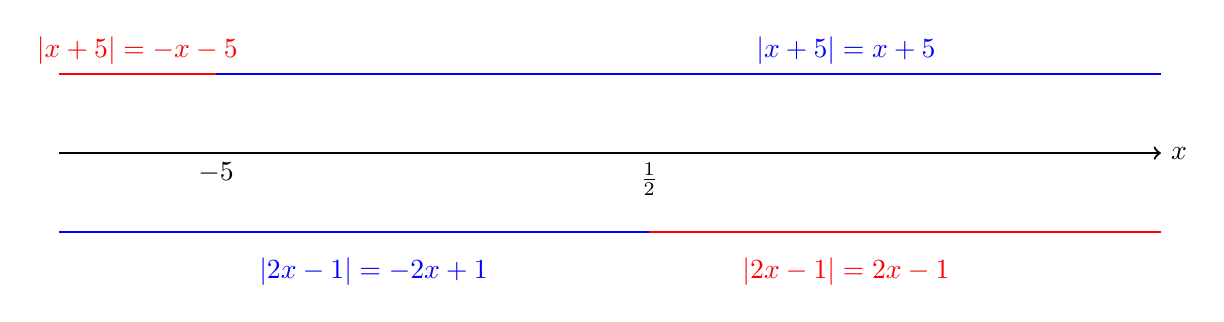
\begin{tikzpicture}[scale=1]
        % Eje horizontal
        \draw[->, thick] (-7,0) -- (7,0) node[right] {$x$};
        
        % Marcas en el eje x
        \draw (-5,0) node[below] {$-5$};
        \draw (0.5,0) node[below] {$\frac{1}{2}$};
        
        % Intervalos
        \draw[red, thick] (-7,1) -- (-5,1);
        \draw[blue, thick] (-5,1) -- (7,1);
        \draw[blue, thick] (-7,-1) -- (0.5,-1);
        \draw[red, thick] (0.5,-1) -- (7,-1);
        
        % Etiquetas mejor ubicadas
        \node[red, above] at (-6,1) {$|x+5|=-x-5$};
        \node[blue, above] at (3,1) {$|x+5|=x+5$};
        \node[blue, below] at (-3,-1.2) {$|2x-1|=-2x+1$};
        \node[red, below] at (3,-1.2) {$|2x-1|=2x-1$};
    \end{tikzpicture}
\end{center}

\subsubsection*{Resolución por casos:}

\textbf{Caso 1}: \(x < -5\)
\begin{align*}
    -(2x-1) - \big[-(x+5)\big] &= 3,\\[1mm]
    -2x+1 + x+5 &= 3,\\[1mm]
    -x+6 &= 3,\\[1mm]
    -x &= -3,\\[1mm]
    x &= 3.
\end{align*}
\textbf{Conclusión}: \(3 \notin (-\infty,-5)\) \quad (\textbf{No es solución})

\textbf{Caso 2}: \(-5 \leq x < \frac{1}{2}\)
\begin{align*}
    -(2x-1) - (x+5) &= 3,\\[1mm]
    -2x+1 - x-5 &= 3,\\[1mm]
    -3x-4 &= 3,\\[1mm]
    -3x &= 7,\\[1mm]
    x &= -\frac{7}{3} \approx -2.33.
\end{align*}
\textbf{Conclusión}: \(-\frac{7}{3} \in \left[-5, \frac{1}{2}\right)\) \quad (\textbf{Solución válida})

\textbf{Caso 3}: \(x \geq \frac{1}{2}\)

\begin{align*}
    (2x-1) - (x+5) &= 3,\\[1mm]
    2x-1 - x-5 &= 3,\\[1mm]
    x-6 &= 3,\\[1mm]
    x &= 9.
\end{align*}

\textbf{Conclusión}: \(9 \in \left[\frac{1}{2}, \infty\right)\) \quad (\textbf{Solución válida})\\
\subsubsection*{Solución general}
\begin{equation*}
    x = \frac{-7}{3} , x = 9
\end{equation*}

\subsubsection*{Interpretación}

La ecuación \(|2x - 1| - |x + 5| = 3\) indica que, para ciertas posiciones de \(x\), la primera distancia $|x-\frac{1}{2}|$ (multiplicada por 2) excede a la segunda distancia en 3 unidades.

Por se hallan los dos puntos específicos: \(\frac{7}{3}\) y $9$ como soluciones.

%%Segunda inecuacion
\subsection*{$|x-1|-|x-3|\geq 5$}
\begin{align*}
    |x-1| &= \begin{cases}
        x-1, & x \geq 1, \\
        -(x-1), & x < 1.
    \end{cases} \\
    |x-3| &= \begin{cases}
        x-3, & x \geq 3, \\
        -(x-3), & x < 3.
    \end{cases}
\end{align*}

\subsubsection*{Gr\'afica de los intervalos}

\begin{center}
    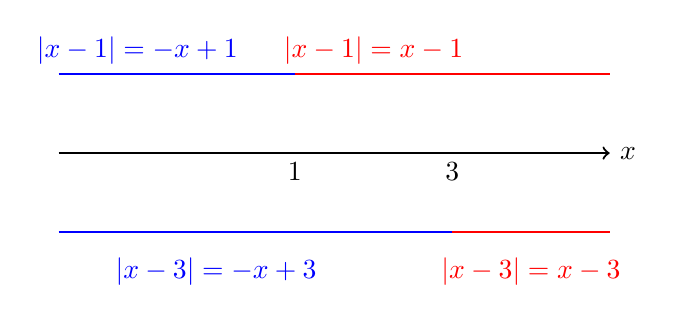
\begin{tikzpicture}[scale=1]
        % Eje horizontal
        \draw[->, thick] (-2,0) -- (5,0) node[right] {$x$};
        
        % Marcas en el eje x
        \draw (1,0) node[below] {$1$};
        \draw (3,0) node[below] {$3$};
        
        % Intervalos
        \draw[blue, thick] (-2,1) -- (1,1);
        \draw[red, thick] (1,1) -- (5,1);
        \draw[blue, thick] (-2,-1) -- (3,-1);
        \draw[red, thick] (3,-1) -- (5,-1);
        
        % Etiquetas mejor ubicadas
        \node[blue, above] at (-1,1) {$|x-1|=-x+1$};
        \node[red, above] at (2,1) {$|x-1|=x-1$};
        \node[blue, below] at (0,-1.2) {$|x-3|=-x+3$};
        \node[red, below] at (4,-1.2) {$|x-3|=x-3$};
    \end{tikzpicture}
    \end{center}
    

\subsubsection*{Resoluci\'on por casos}

\textbf{Caso 1}: $x < 1$
\begin{align*}
    (-x+1) - (-x+3) &\geq 5,\\
    -x+1 + x -3 &\geq 5,\\
    -2 &\geq 5.
\end{align*}
\textbf{Conclusi\'on}: Falso \quad (\textbf{No hay soluci\'on})

\textbf{Caso 2}: $1 \leq x < 3$
\begin{align*}
    (-x+3) - (x-1) &\geq 5,\\
    -x+3 - x +1 &\geq 5,\\
    -2x +4 &\geq 5,\\
    -2x &\geq 1,\\
    x &\leq -\frac{1}{2}.
\end{align*}
\textbf{Conclusi\'on}: $-\frac{1}{2} \notin [1,3)$ \quad (\textbf{No hay soluci\'on})

\textbf{Caso 3}: $x \geq 3$
\begin{align*}
    (x-3) - (x-1) &\geq 5,\\
    x-3 - x +1 &\geq 5,\\
    -2 &\geq 5.
\end{align*}
\textbf{Conclusi\'on}: Falso \quad (\textbf{No hay soluci\'on})

\subsubsection*{Soluci\'on general}

\begin{equation*}
    \text{No hay soluciones reales.}
\end{equation*}


\subsubsection*{Interpretación}
Esta inecuación indica que no hay valores de $x$ que cumplan con la condición de que la diferencia de que la distancia entre $x$ y $1$ sea mayor o igual a la distancia entre $x$ y $3$ en 5 unidades.

%%Tercera inecuacion
\subsection*{$|x^2-1|\leq \frac{1}{2}$}

\[-\frac{1}{2} \leq x^2 - 1 \leq \frac{1}{2}\]

\subsubsection*{Primera desigualdad}
\[-\frac{1}{2} \leq x^2 - 1\]
\[-\frac{1}{2} + 1 \leq x^2\]
\[\frac{1}{2} \leq x^2\]
\[|x| \geq \sqrt{\frac{1}{2}}\]
\[x \leq -\sqrt{\frac{1}{2}} \quad \text{ó} \quad x \geq \sqrt{\frac{1}{2}}\]

\subsubsection*{Segunda desigualdad}

\[x^2 - 1 \leq \frac{1}{2}\]
\[x^2 \leq \frac{1}{2} + 1\]
\[x^2 \leq \frac{3}{2}\]
\[|x| \leq \sqrt{\frac{3}{2}}\]
\[-\sqrt{\frac{3}{2}} \leq x \leq \sqrt{\frac{3}{2}}\]

\subsubsection*{Gráfica de los intervalos}
\begin{center}
    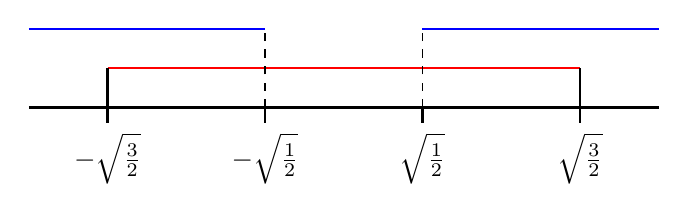
\begin{tikzpicture}
        % Eje
        \draw[thick] (-4,0) -- (4,0);
        
        % Puntos en la recta con etiquetas corregidas
        \draw[thick] (-3,0) --++ (0,-0.2);
        \node[below] at (-3,-0.2) {$-\sqrt{\frac{3}{2}}$};
    
        \draw[thick] (-1,0) --++ (0,-0.2);
        \node[below] at (-1,-0.2) {$-\sqrt{\frac{1}{2}}$};
    
        \draw[thick] (1,0) --++ (0,-0.2);
        \node[below] at (1,-0.2) {$\sqrt{\frac{1}{2}}$};
    
        \draw[thick] (3,0) --++ (0,-0.2);
        \node[below] at (3,-0.2) {$\sqrt{\frac{3}{2}}$};
    
        % Intervalo cerrado en rojo (-sqrt(3/2), sqrt(3/2))
        \draw[thick, red] (-3,0.5) -- (3,0.5);
        \draw[thick] (-3,0) -- (-3,0.5);
        \draw[thick] (3,0) -- (3,0.5);
        
        % Intervalos abiertos en azul (-∞, -sqrt(1/2)) y (sqrt(1/2), ∞)
        \draw[thick, blue] (-4,1) -- (-1,1);
        \draw[thick, blue] (1,1) -- (4,1);
        \draw[dashed] (-1,0) -- (-1,1);
        \draw[dashed] (1,0) -- (1,1);
        
    \end{tikzpicture}
\end{center}

\subsubsection*{Solución:} 
\begin{equation*}
    x \in \left[-\sqrt{\frac{3}{2}}, -\sqrt{\frac{1}{2}}\right] \cup \left[\sqrt{\frac{1}{2}}, \sqrt{\frac{3}{2}}\right].
\end{equation*}

\subsubsection*{Interpretación}
Esta inecuacion indica que los valores de $x$ que cumplen con la condición de que la distancia entre $x^2$ y $1$ sea menor o igual a $\frac{1}{2}$ son aquellos que se encuentran en el intervalo $[-\sqrt{\frac{3}{2}}, -\sqrt{\frac{1}{2}}] \cup [\sqrt{\frac{1}{2}}, \sqrt{\frac{3}{2}}]$.
\section{Límites y Derivadas}

\begin{enumerate}
    \item $ \lim\limits_{x \to 2} \frac{x^2 - 4}{x - 2} $
    
    \textbf{Caso: Diferencia de Cuadrados}
    \[ \lim\limits_{x \to 2} \frac{(x+2)(x-2)}{x-2} = \lim\limits_{x \to 2} x+2 = 4 \]
    
    \item $ \lim\limits_{x \to 0} \frac{\sin x}{x} $
    
    \textbf{Regla de L'Hôpital}
    \[ \lim\limits_{x \to a} \frac{f(x)}{g(x)} = \lim\limits_{x \to a} \frac{f'(x)}{g'(x)} \]
    Para los casos $ \frac{0}{0} $ o $ \frac{\infty}{\infty} $:
    \[ \lim\limits_{x \to 0} \frac{\cos x}{1} = \frac{1}{1} = 1 \]
    
    \item $ \lim\limits_{x \to \infty} \frac{3x^2 + 5}{2x^2 - 7} $
    
    \textbf{Se divide todo por el mayor exponente}
    \[ \lim\limits_{x \to \infty} \frac{K}{x^n} = 0 \]
    
    \[ \lim\limits_{x \to \infty} \frac{\frac{3x^2}{x^2} + \frac{5}{x^2}}{\frac{2x^2}{x^2} - \frac{7}{x^2}} = \frac{3 + 0}{2 - 0} = \frac{3}{2} = 1.5 \]
    
\end{enumerate}

\section*{Cálculo de Derivadas}

Calcule la derivada de las siguientes funciones:

\begin{enumerate}
    \item \( f(x) = x^3 - 4x + 2 \)
    
    \[
    f'(x) = 3x^2 - 4
    \]

    \item \( g(x) = e^x \sin x \)
    
    \[
    g'(x) = e^x \sin x + e^x \cos x
    \]
    
    \[
    g'(x) = e^x (\sin x + \cos x)
    \]

    \item \( h(x) = \ln(x^2 + 1) \)
    
    \textbf{Regla de la cadena:}
    
    \[
    \frac{d}{dx} \ln u = \frac{1}{u} \cdot u'
    \]
    
    \[
    h'(x) = \frac{2x}{x^2 + 1}
    \]
\end{enumerate}
\section{Problemas Rutinarios}

Se espera que las siguientes actividades le permitan comprender, repasar y utilizar propiedades y métodos analíticos que aprendió en el curso de Cálculo Diferencial:

\begin{enumerate}
    \item Determine la ecuación de la recta tangente a la función \(f(x)=x^2+3x-5\) en \(x=1\).
    \item Encuentre los puntos críticos y clasifíquelos como máximos, mínimos o puntos de silla para la función \(f(x)=x^3-6x^2+9x+2\).
    \item Analice la continuidad de la función:
    $$
    f(x)=\begin{cases}
    x^2-1, & x<2, \\
    3x-5, & x\geq 2.
    \end{cases}
    $$
    \item Use herramientas de cálculo para hacer un \emph{sketch} de la gráfica de las siguientes funciones, además, describa el paso a paso para llegar a su \emph{sketch}:
    \begin{enumerate}
        \item \(f(x)=\frac{x}{x^2-1}\),
        \item \(f(x)=\frac{1}{(x-1)(x-3)}\),
        \item \(f(x)=x+\frac{1}{x^2}\).
    \end{enumerate}
\end{enumerate}
\section{Lectura, Escritura y Exposición}
Leer y hacer un resumen conciso de las sesiones 1.1, 1.2 y 1.3 de [4].
\section{Problemas No Rutinarios}

Si \(f\) es una función continua en un intervalo cerrado \([a, b]\), excepto quizás en un punto \(c\in[a,b]\), determine la veracidad o falsedad de los siguientes enunciados (justifique su respuesta):

\begin{itemize}
    \item Si \(f'(x)\) es positiva para todo \(x<c\), y \(f'(x)\) es negativa para todo \(x>c\), en el punto \(c\) hay un máximo relativo de \(f\).
\end{itemize}

El enunciado en pocas palabras establece que si que a la izquierda de $c$ la función es creciente  ($f'(x) > 0$ para $x < c$) y a la derecha de $c$ es decreciente  ($f'(x) < 0$ para $x > c$) , entonces hay un máximo relativo. Esto no es cierto porque la función debe ser continua en todo el intervalo $[a, b]$, si $c \in [a, b]$ entonces la función no tiene un punto crítico. El criterio de la primera derivada dice que para analizar el crecimiento de una función es necesario calcular en qué casos dicha derivada vale cero o no existe.

Hay que tener en cuenta de que si una función crece a la izquierda y decrece a la derecha de $c$ o viceversa, no significa siempre que exista un máximo o un mínimo relativo en $[a, b]$ de $f$, pues puede darse el caso de que en $c$ existan asíntotas como se aprecia en la función racional de la figura \ref{fig:racional1}. Un punto crítico es donde la derivada de la función es cero, sin embargo puede existir un punto de discontinuidad, allí la derivada no existe, pero puede crecer o decrecer sin necesidad de ser un máximo o un mínimo.

En cambio, en la función cuadrática de la figura \ref{fig:cuadratica1} no hay una asíntota y aparentemente es un máximo, pero no lo es porque allí la derivada no existe. \textbf{Por lo tanto el enunciado es falso}.

\begin{figure}[H]
    \centering
    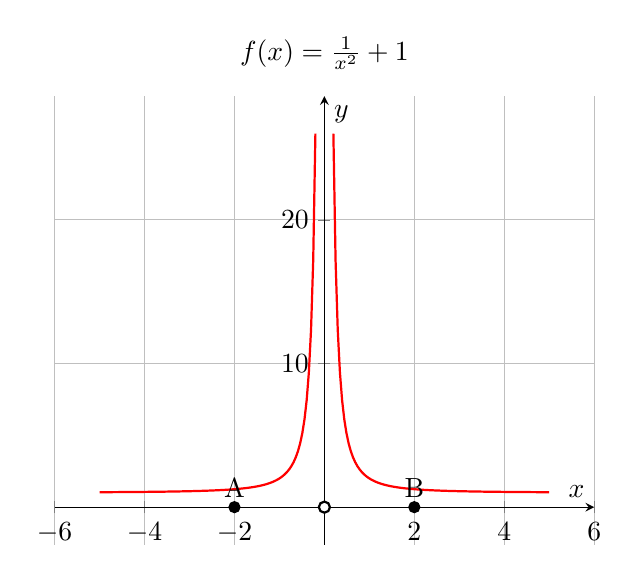
\begin{tikzpicture}
    \begin{axis}[
        title={$f(x) = \frac{1}{x^2} + 1$},
        axis lines = middle,
        grid = major,
        enlargelimits = true,
        xlabel={$x$},
        ylabel={$y$},
    ]
    
    % Función racional
    \addplot[domain=-5:-0.2, samples=100, thick, red] {((1)/(x^(2)))+1};
    \addplot[domain=0.2:5, samples=100, thick, red] {((1)/(x^(2)))+1};
    
    % Puntos marcados
    \addplot[only marks, mark=*, mark options={black}, nodes near coords={A}] coordinates {(-2,0)};
    \addplot[only marks, mark=*, mark options={black}, nodes near coords={B}] coordinates {(2,0)};
    \addplot[only marks, mark=*, mark options={white}, scale=1.5] coordinates {(0,0)};
    \addplot[only marks, mark=o, mark options={black}, scale=1.5, thick] coordinates {(0,0)};
    
    \end{axis}
\end{tikzpicture}
    \caption{Función racional decreciente y creciente antes y después de $c$ respectivamente.}
    \label{fig:racional1}
\end{figure}

\begin{figure}[H]
    \centering
    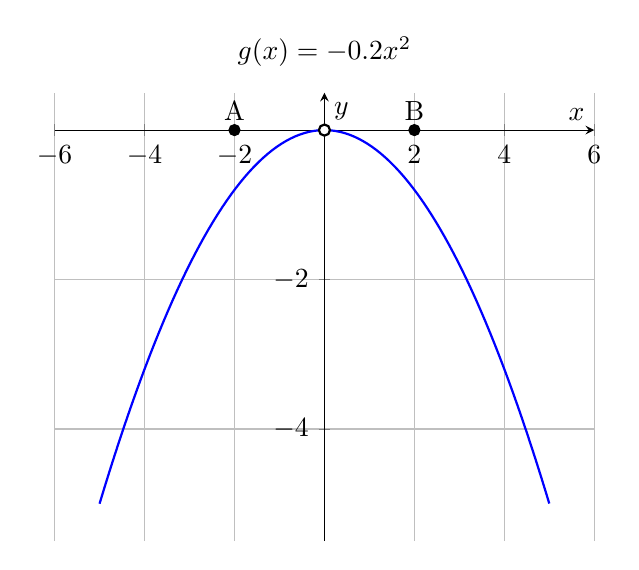
\begin{tikzpicture}
    \begin{axis}[
        title={$g(x) = -0.2x^2$},
        axis lines = middle,
        grid = major,
        enlargelimits = true,
        xlabel={$x$},
        ylabel={$y$},
    ]
    
    % Función cuadrática
    \addplot[domain=-5:5, samples=100, thick, blue] {-0.2*x^2};
    
    % Puntos marcados
    \addplot[only marks, mark=*, mark options={black}, nodes near coords={A}] coordinates {(-2,0)};
    \addplot[only marks, mark=*, mark options={black}, nodes near coords={B}] coordinates {(2,0)};
    \addplot[only marks, mark=*, mark options={white}, scale=1.5] coordinates {(0,0)};
    \addplot[only marks, mark=o, mark options={black}, scale=1.5, thick] coordinates {(0,0)};
    
    \end{axis}
\end{tikzpicture}
    \caption{Función cuadrática decreciente y creciente antes y después de $c$ respectivamente.}
    \label{fig:cuadratica1}
\end{figure}

\begin{itemize}
    \item Si \(f'(x)\) es negativa para todo \(x<c\), y \(f'(x)\) es positiva para todo \(x>c\), en el punto \(c\) hay un mínimo relativo de \(f\).
\end{itemize}

En este enunciado se podría aplicar la misma lógica que en el primero, pero abordaré en este el criterio de la segunda derivada. Una vez se hallan los puntos críticos igualando la primera derivada a cero, entonces se evavlúa la segunda derivada en dichos puntos y si $f''(x) > 0$ entonces la función es cóncava hacia arriba y si $f''(x) < 0$ entonces la función es cóncava hacia abajo.

Si la función es cóncava hacia arriba en un punto crítico, entonces es un mínimo relativo y si es cóncava hacia abajo, entonces es un máximo relativo. Sin embargo, en este caso no existen puntos críticos, ya que al igualar $f'(x) = 0$ no se obtiene ninguna solución. \textbf{Por lo tanto, el enunciado es falso}.

En las siguientes gráficas se puede apreciar lo anteriormente mencionado:

\begin{figure}[H]
    \centering
    \input{images/noRutinarios1,3.tex}
    \caption{Función racional creciente y decreciente antes y después de $c$ respectivamente.}
    \label{fig:racional2}
\end{figure}

\begin{figure}[H]
    \centering
    \input{images/noRutinarios1,4.tex}
    \caption{Función cuadrática creciente y decreciente antes y después de $c$ respectivamente.}
    \label{fig:cuadratica2}
\end{figure}
\section{Análisis Numérico o Computacional}

\begin{enumerate}
    \item Use el método de la bisección para encontrar una aproximación a la raíz de la ecuación \(f(x)=x^3-x-2\) en el intervalo \([1,2]\) con una tolerancia de \(10^{-3}\).
    \item Aproxime la derivada de \(f(x)=e^x\) en \(x=1\) usando diferencias finitas progresivas con \(h=0.1\).
\end{enumerate}Función racional creciente y decreciente antes y después de $c$ respectivamente.

\begin{thebibliography}{9}
    \bibitem{1} Stewart J. -- \emph{Calculus Concepts and Contexts}, 2ª ed., Thomson (2004).
    \bibitem{2} Boyce, W. E.; DiPrima, R. C.; Meade, D. B. -- \emph{Elementary Differential Equations and Boundary Value Problems}, Wiley (2021).
    \bibitem{3} Marsden, J.; Tromba, A. -- \emph{Cálculo Vectorial}, (1991).
    \bibitem{4} Apostol, T. -- \emph{Calculus Volumen I: Cálculo con funciones de una variable, con una introducción al álgebra lineal}, 2ª ed., Reverte (2001).
\end{thebibliography}

\end{document}